\chapter[Introduction]{Introduction}
\label{Chap:Intro}

% ***************************************************
% Introduction
% ***************************************************

\section{Background and motivation}

\subsection{Biology background of cellular communication}
Cell-cell communication is mechanisms that enable one cell to influence the behavior of itself or another cell to ultimately coordinate biological processes to response the changes in intracellular and extracellular environment. It is vital for individual cells to be able to communicate with each other and their environment as a part of a functional multicellular organism to enable higher-order biological processes. For example, during embryonic development, cells differentiate into complex tissues and organs and these fate decisions are controlled through communications with neighboring cells \cite{gale1996eph, eichmann1997ligand}. Responses of immune cells against pathogens or tumours cells is another example of the cell-cell communication. When these signals are missing (i.e. in vitro), certain cell types enter a suicide program known as apoptosis (Figure \ref{fig:Chap1_figure1}). 

By studying cell communication, we can systematically understand coordinated cellular behaviors and unravel complex extracellular responses. Cell behaviors which consist of different complex processes are governed by specific combinations of extracellular signals (multiple ligands) rather than a single signal alone (Figure \ref{fig:Chap1_figure1}A-C). Each cell has been programmed to respond to a specific set of extracellular signals to survive and perform specialised functions. Each cell often requires multiple signals to survive (Figure \ref{fig:Chap1_figure1}A) or grow and divide (Figure \ref{fig:Chap1_figure1}B). Some signals can induce the changes in cells outward behaviours or appearance such as cell differentiation (Figure \ref{fig:Chap1_figure1}C). If deprived of appropriate survival signals, a normal cell will activate the apoptosis process (Figure \ref{fig:Chap1_figure1}D). The mechanisms behind cell communication commonly involve the combinations of extracellular proteins called ligands and transmembrane proteins called receptors \cite{alberts2018molecular}. Even with the same set of signals, distinct cell types can respond differently as the responses of the cells also rely on the combination of receptor proteins that they possess. There are thousands of ligand-receptor pairs that have been curated over the last decade \cite{salwinski2004database, orchard2012protein} and the number of signalling combinations and responses is almost infinite.

\begin{figure}[htp]
% \renewcommand{\figurename}{Supplementary Figure}
    \centering
    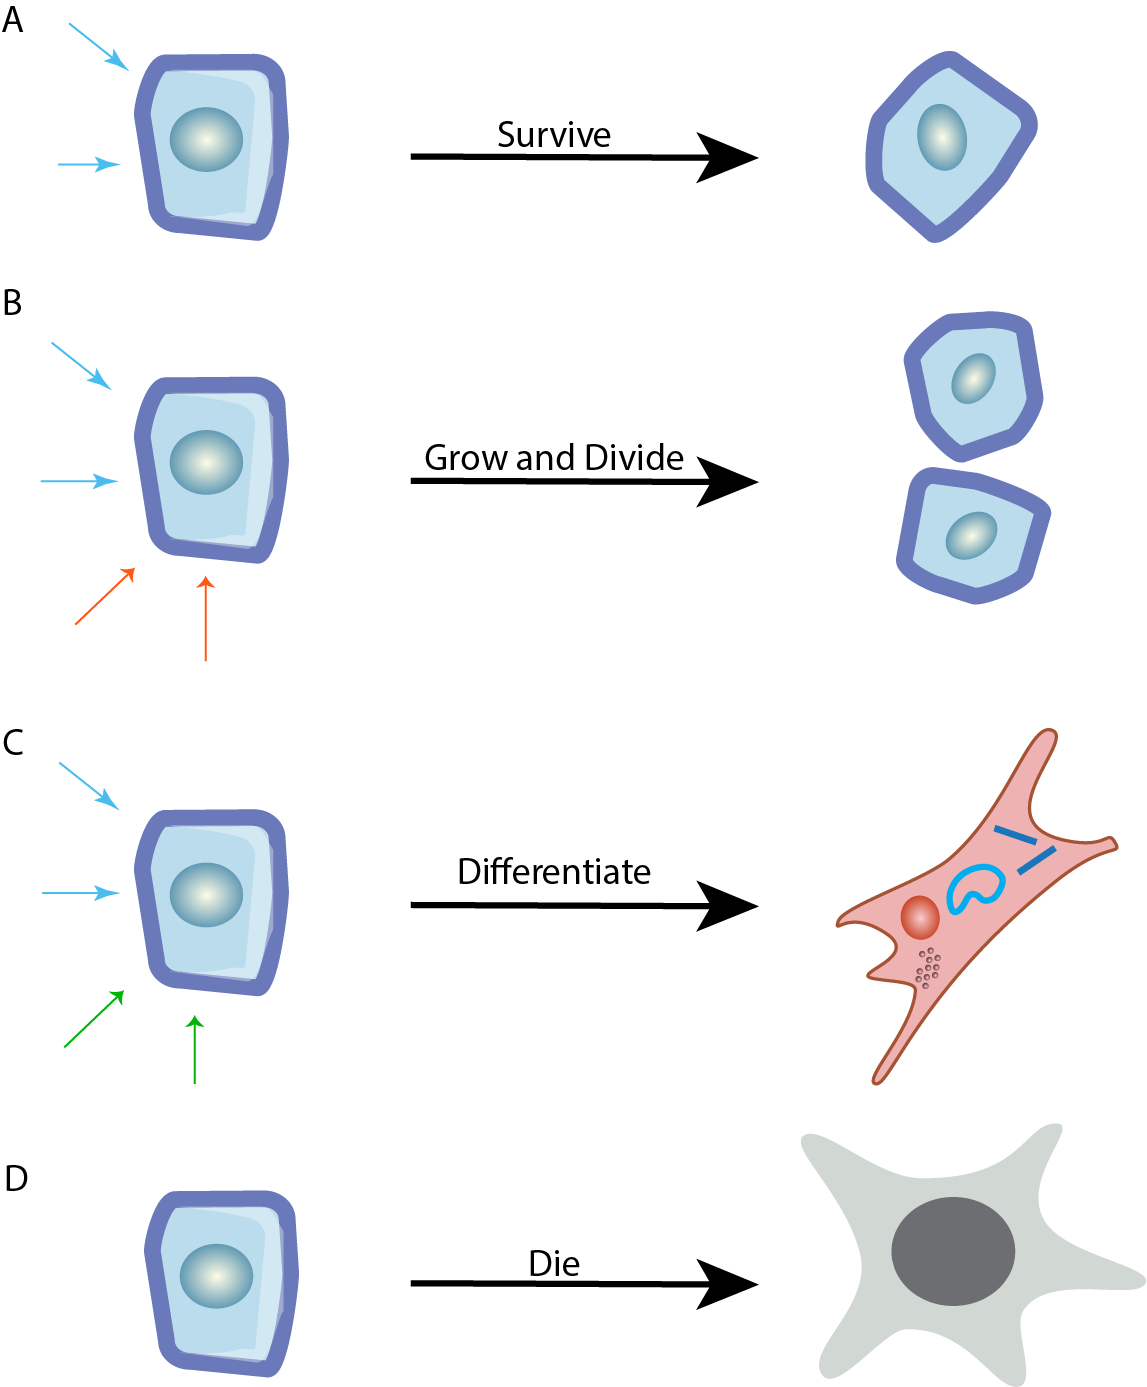
\includegraphics[width=0.6\columnwidth]{Chapter1/Figures/Chap1_figure1.png}
    \caption{Cell relies on multiple extracellular signaling molecules to survive. A cell can receive and response to the signaling molecules produced by other cells using a set of receptors. The behaviors of a cell varied depends on type of signals including (A) survive (blue arrows), (B) signals to grow and divide (red arrows) or (C) differentiate (green arrows). (D) Absence of survival signals, can induce of cell suicide program known as apoptosis}
    \label{fig:Chap1_figure1}
\end{figure}

It is natural to make an analogy between the cell signalling systems and a human social organisation. The organisation relies on the collaboration and coordination from multiple department to operate functionally. The well-being of the individual is often set to lower the benefit of the whole. Similarly, cells in the multicellular organisms heavily rely on the interaction between individuals to be functional \cite{bartee2018principles}. Through advances in computational biology and experimental throughput, we can now intensively characterise these signaling mechanisms and even simulate the cell-cell signalling networks to better understand the principles of how the interactions between cells can drive biological function \cite{sprinzak2010cis, teague2016synthetic, toda2019engineering}. Furthermore, technology development enables us to conduct more experiments in cells within living organisms \cite{helmchen2005deep, periasamy2013methods}, and spawns new means to study the cell microenvironment within tissue context. 

Before discussing about the approaches to study cell-cell interaction in their spatial proximity, it is reasonable to revisit the major types of communications that the cells can perform. To perform the communication, cell secrete signaling molecules to outside of cell's membrane. The molecules can transmit through short or long distance bind to the receptors at the surface of target cell's membrane. Some signaling molecules are very small and unstable that required two cell's membranes to be in contact to exchange signals. However, in most cases, the signaling molecules can travel to distant cells in which the gradient of factor received can determine the behaviours.         

The contact-dependent interaction between cells, which two cells are physically in contact called \textit{gap junctions}. These are specialized intercellular connections that link the cytoplasm of two adjacent cells via narrow filled channels (Figure \ref{fig:Chap1_figure2}A). The channels allow cells to exchange various small molecules, ions but not macro-molecules, such as proteins or nucleic acids. Studies show that communication through gap junctions plays crucial roles in cell synchronization, differentiation, embryonic development, and immune response \cite{white1999genetic, vinken2006connexins}. For example, severe defects in heart development were found in mouse embryos to be caused by the mutation of one particular gap-junction protein (connexin 43)

While gap junctions are contact-dependent communications and allow cells to exchange ions or second messengers, cell communication also can take place across near or long distances. In most cases, signaling molecules are secreted to outside of the membrane of signaling cells which act as local mediators, affecting neighboring cells in the immediate environment. Alternatively, the signaling molecules can also transmit through the circulation to act on target cells at far distant sites \cite{cooper2004cell, alberts2018molecular}. The former signaling pathway when molecules are transmitted via a local distance is called \textit{paracrine signalling}. In paracrine signalling, cells secrete signaling molecules called ligands and induce changes in nearby cells (Figure \ref{fig:Chap1_figure2}B). The ligand molecules in paracrine signalling tend to be rapidly absorbed by neighboring target cells; destroyed by extracellular enzymes, or immobilized by the extracellular matrix. Prominent examples of paracrine signalling systems include neurotransmitters between nerve cells at a synapse,  blood clotting system, tissue repair, and formation of scars
\cite{huang1998gap}. 

The alternative form of distant signalling when the molecules travel through the extracellular fluids to reach to receiver cells called \textit{endocrine signalling}. Endocrine cells secrete their signaling molecules in the form of hormones, into the blood circulation, which sends the signal to targets cell throughout the body (Figure \ref{fig:Chap1_figure2}C). Signal transmission in endocrine systems is much slower than in paracrine signalling and tends to last for longer as it relies on diffusion and blood flow. One classic example is pancreatic cells producing the hormone insulin which signals cells in fat, muscles, and liver to absorb glucose and maintain blood sugar levels.

\begin{figure}[htp]
% \renewcommand{\figurename}{Supplementary Figure}
    \centering
    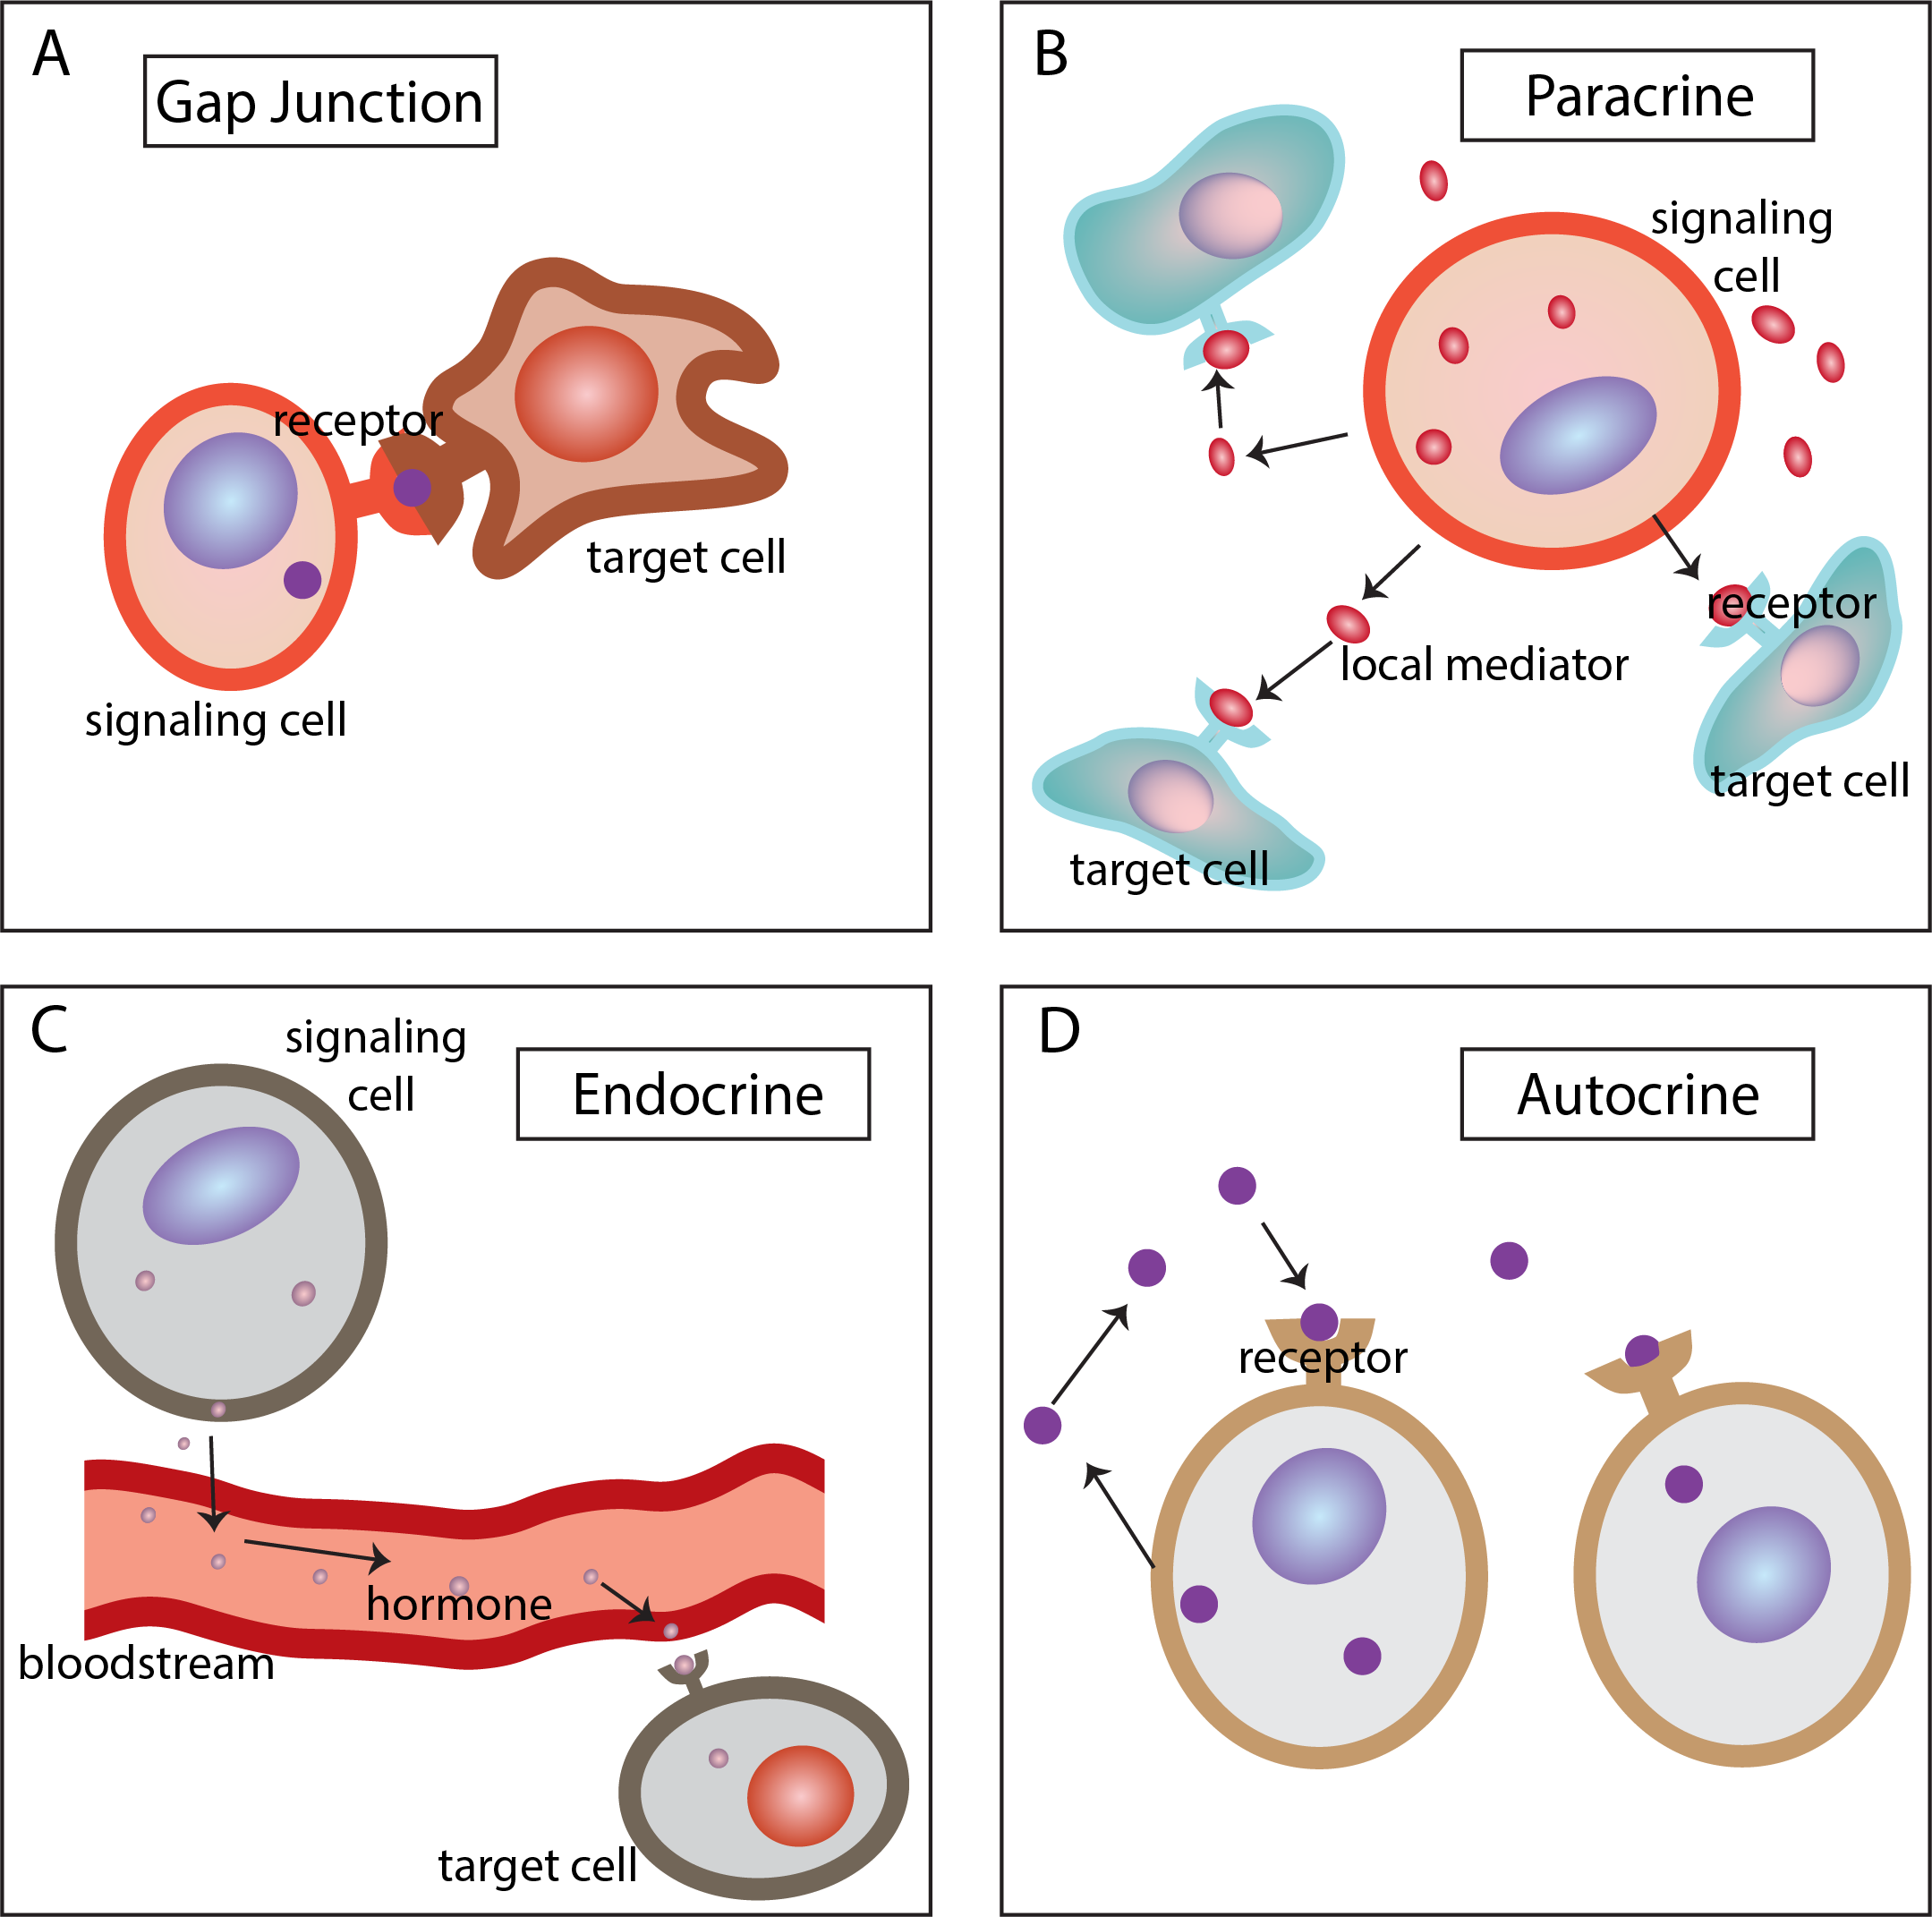
\includegraphics[width=0.8\columnwidth]{Chapter1/Figures/Chap1_figure2.png}
    \caption{4 Type of cell-cell interactions (A) Gap junctions is contact-dependent signaling which requires cells to be in membrane–membrane contact. (B) Paracrine signaling does not require membrane-membrane contact, rather depending on local mediating signaling molecules that are released into the extracellular space and act on neighboring cells. (C) Endocrine signaling depends on endocrine cells, which secrete hormones into the bloodstream for distribution throughout the body. (D) Autocrine signaling refers to cells secrete signaling molecules to induce the changes of the same cells}
    \label{fig:Chap1_figure2}
\end{figure}

Some cells can secrete signaling molecules to self-regulate or to control other neighboring cells of the same type. This type of communication is called \textit{autocrine signalling}. In \textit{autocrine signalling} (or intracrine signalling), cells stimulate themselves by sending the signaling molecules and back to their own receptors. Autocrine signalling is most effective when occurring within the same cell or with neighboring cells of the same type (Figure \ref{fig:Chap1_figure2}D). The process is used to encourage groups of cells to make the same developmental decision. Thus, autocrine signalling is often found in cells that are differentiated along a particular pathway to reinforce developmental decisions \cite{alberts2018molecular}. Autocrine signalling is often found in cancer cells and enhances cell differentiation and proliferation \cite{sporn1985autocrine}.  

Every kind of cell, from the bacterium to sophisticated eukaryotic cell, can secrete the chemical signals to perform cellular communication. The mechanism of cell signalling in single-cellular organisms such as yeast and bacteria has been well studied and understood \cite{alberts2018molecular}. Meanwhile, during the evolution of multicellular organisms, the signaling among cells achieved a high level of complexity. The crosstalks between different cell types from multiple tissues which is crucial to every organisms, forms a complex microenvironment system to govern tissue functions. This is not only because the signaling methods are complex, it is also because the quantity of cells present in the microenvironment can drive interaction to different outcomes. It is much more difficult to study the microenvironment system as a whole without a quantitative analysis and computational methods. Therefore, this thesis will hereinafter discuss only cell signalling in multicellular organisms, especially human and demonstrate the robustness of quantitative approaches to uncover the cellular communication system. 

\subsection{The biology process of cancer}
In all multicellular organisms, each individual cell is a part of the whole community and follows behaves in a socially responsible manner. To remain the balance of the harmony of the society, the number of cells in an adult body remain constant (around $10^{14}$ cells in human). However, throughout the lifespan, a cell can acquire some mutations which allow it to keep growing and dividing than its neighboring cells \cite{alberts2018molecular, greaves2012clonal}. Most of mutated cells will be detected and either repaired or eliminated by the immune surveillance system in the body. However, cancer cells are said to be genetically unstable cells that accumulate enough mutations which give them \textbf{malignant} properties to break immunosurveillance and invade surrounding tissue. 

There are two malignant properties a cell need to possess to be classified cancer cell. The cell needs to develop the mutations that allow it to (1) reproduce at abnormally speed, and (2) be able to invade and colonize tissue sites normally reserved for other cells. An abnormal cell that either increases in size or proliferates out of control will give rise to a neoplasm \cite{alberts2018molecular, hanahan2000hallmarks}. The combination of the two properties that contributes to the fatality cancers. As long as the neoplastic cells have not yet become invasive, the tumour is considered as \textbf{benign}. A tumor is considered as \textbf{malignant} when its cells have developed the ability to invade neighbouring tissue. The metastability is a dangerous characteristic of cancer cells. It even allows cancer cells to migrate to other part of the body through blood stream or lymphatic vessels, and form secondary tumours \cite{alberts2018molecular}. The further a cancer cell metastasises the more resistant to eradication it becomes.   

The abnormal reproduction of cells foster tumour progression and tumorigenesis. Most normal cells in the body have the built-in safety mechanisms which limits number of successive cell growth-and-division cycles (Figure \ref{fig:Chap1_figure3}) \cite{hanahan2000hallmarks, hanahan2011hallmarksnext}. This safety mechanisms consist of two distinct barriers: \textbf{senescence}, a typically irreversible entrance into a non-proliferative but viable state; and apoptosis, which involves cell death (Figure \ref{fig:Chap1_figure3}A). Cancer cells are found to contain the mutations that can disable normal safety mechanisms which is either an increase in cell division or an inhibition of apoptosis. In addition to the capability to alter built-in cell senescence and/or cell apoptosis, cancer cells also very resistant to cell stress an DNA damage. The tumour grows because the cell birth rate outweight the cell death rate, but often by only a small margin (Figure \ref{fig:Chap1_figure3}B-C). Therefore, the time that a tumour takes to double in size is only a gradual process.

\begin{figure}[htp]
% \renewcommand{\figurename}{Supplementary Figure}
    \centering
    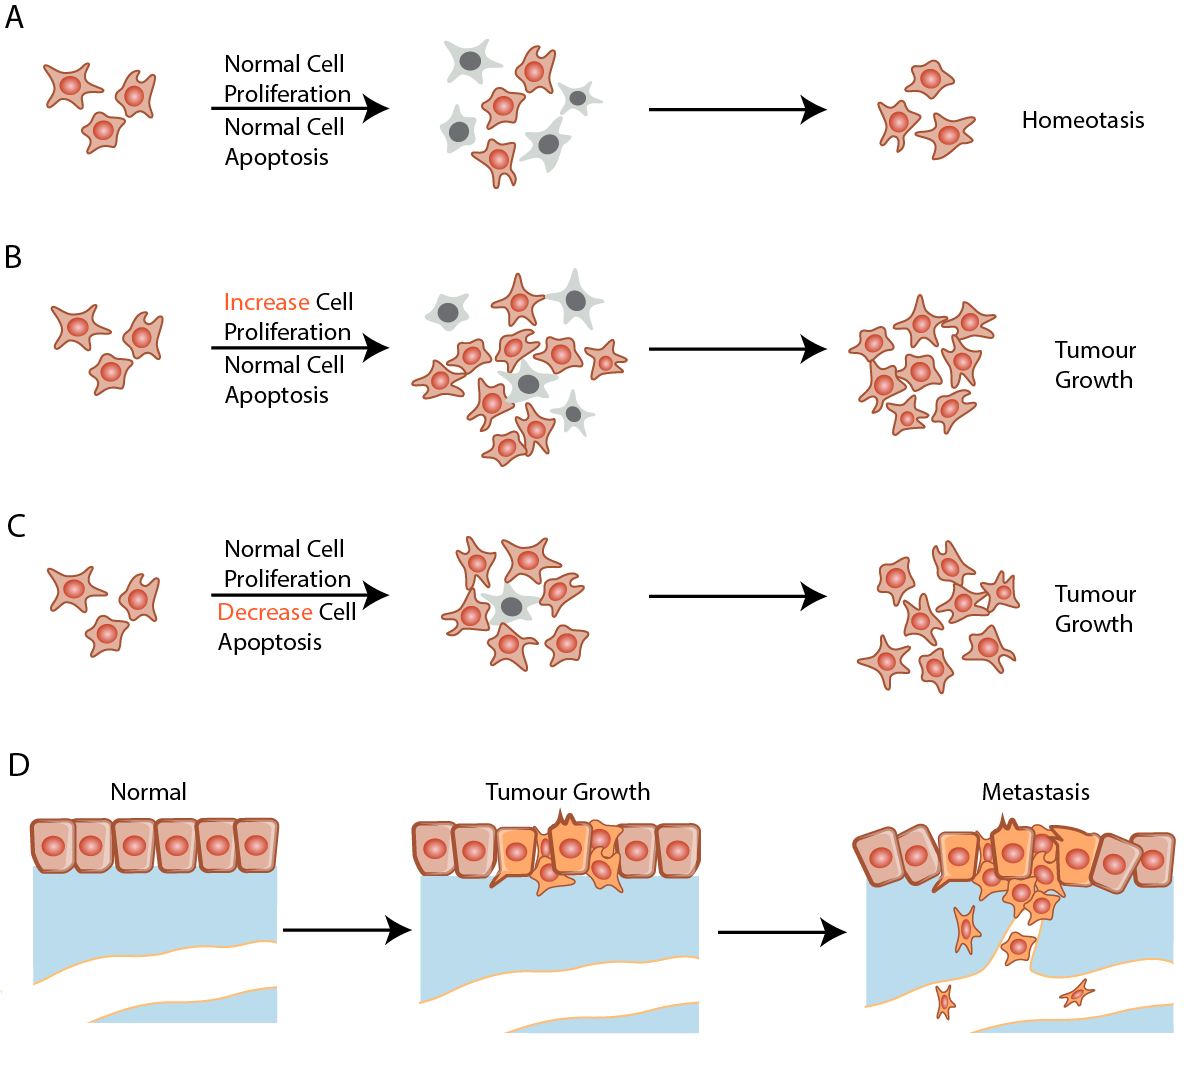
\includegraphics[width=0.7\columnwidth]{Chapter1/Figures/Chap1_figure3.png}
    \caption{Tumorigenesis and metastasis process. The development of a tumour is the result the mutated cells acquired either stronger cell proliferation or inhibition of apoptosis (A-C). (D) An illustration of tumour cells reside from an organ to other organs through the bloodstream (figure adapted from \cite{alberts2018molecular})}
    \label{fig:Chap1_figure3}
\end{figure}

Metastasis is, in fact, a multistep process where cancer cells first invade locally, migrate to the circulation (lymphatics or bloodstream), and finally establish the new tumor at distant organism. Cancer cell is dangerous due to its invasiveness and the ability to break free of constraints that keep normal cells in their designated organ \cite{greaves2012clonal}. Such properties is often acquired by the disorganized pattern of tumour growth and ragged borders, invading into the neighbouring tissue. Fewer than one in thousand of malignant tumour cells that enter bloodstream will colonise in a new organ and grow to the detectable secondary tumours \cite{joyce2009microenvironmental}. With modern blood test techniques, cancer cells can be early detected according to their surface properties while circulating in samples of blood from cancer patients. These biomarker can inform the early treatment (\ie TP53, APC in colorectal cancer \cite{markowitz2009molecular}). 

While cancer cells tend to avoid apoptosis, this does not mean that they are immortal. In the interior of a large solid tumour, cell death often occurs on a massive scale. However, cancer cells within the tumour often die from necrosis process, which is unregulated death as the result of environmental perturbations. In necrosis, the cells become bloated and explodes, releasing its contents into the local tissue microenvironment \cite{hanahan2011hallmarksnext}. Tumour necrosis factor (TNF$\alpha$) induce the upregulation of S100A8 and S100A9 in myeloid cells, which can increase the metastasis \cite{hiratsuka2008s100a8, hiratsuka2006tumour}. 

The dynamic of genetic mutations within cell is the major cause of the tumour initiation. However, it is generally agreed that cancer metastasis is partially constrained by a complex, multifactorial interplay between cancer cells and the host tissue microenvironment. Some microenvironmental features can promote neoplastic cells including infiltrating macrophages and neovascularization. Mathematical modeling is an ideal approach to dissect mechanisms of cancer invasion as it can simultaneously and quantitatively consider interactions between multiple factors \cite{anderson2006tumor}. The following sections will discuss deeper about different type of interaction within the cancer and aim to address the need for a computational approach.       

\subsection{The role of cell-cell interaction within cancer microenvironment}
It is often known that cancer originates from genetic instability. However, the growth of cancer cells into the tumour and the process of cancer metastasis are constrained by cellular interaction and tissue spatial conditions that dictate the interaction within and surround the cancer nest \cite{west2019cellular, liotta2001microenvironment,anderson2006tumor}. Cancer cells can produce growth factor ligands themselves, to which they can respond via the expression of cognate receptors resulting in autocrine proliferative stimulation. Many epithelium cells in breast cancer can produce its family of epidermal growth factor (EGF) ligands stimulate cancer cell proliferation and motility, suggesting they may participate in autocrine and signaling with cells of the tumour microenvironment \cite{nickerson2013autocrine}.  

Cancer clone habitats are not closed systems \cite{greaves2012clonal}. Tumours consist of not only cancer cells but also endothelial cells, smooth muscle, fibroblasts and inflammatory white blood cells. Cancer cells in a tumour are the group of cells that accumulated dangerous mutations, however, the development of a tumour relies on a two-way communication between the tumour cells and the surrounding environment (tumour stroma). In cancer pathology studies, tumour microenvironment can influence cancer development in different way. During early tumour development, the protection of the microenvironment surround the tumour foster the tumour growth conditions such as chronic inflammation. As the cancer progress, the cancer cells secrete signal proteins such as TGF-$\beta$ and EGF to stimulate normal cells within to induce epithelial development as well as to modify the extracellular matrix \cite{beck2011systematic,BREMNES2011209}. The stroma, in turn, secrete signal proteins that stimulate cancer cells growth and division (i.e. CXCL12) \cite{kumar2018analysis,wang2017role}. There is a feedback loop of cell-cell interaction between the cancer cell migration and the tissue microenvironments; in which the increase in intratumour cell-cell interaction promotes collective migration in cancer \cite{friedl2011cancer, whiteside2008tumor}, leading to dynamically induced the disorganization of nearby microenvironments of the tissue \cite{friedl2012classifying, canel2013cadherin, almendro2013cellular, roussos2011chemotaxis, zervantonakis2012three}. The prediction of tumour stroma and cancer cell crosstalk has created a type therapeutic strategy which aim to block cancer cells interactions with the environments to create the growth fostering habitat called "ecological therapy" \cite{pienta2008ecological, calabrese2007perivascular, bissell2011don}.      

Crosstalk between cancer and immune cells is also closely connected to the tumourigenesis process including: initiation, progression, and metastasis \cite{wang2017role}. The role of the immune system is to protect the host from infectious pathogens and remove damaged cells \cite{davis2007molecular}. In the early stage of cancer progression, immune cells such as macrophages and myeloid secrete signalling molecules (paracrine or/and endocrine) to trigger a cell apoptosis process to eliminate cancer cells \cite{wyckoff2007direct}. If cancer cells are completely cleared during this elimination stage, immune cells will distribute around the cancer cells to suppress tumour growth \cite{bronkhorst2011detection, ly2010aged}. Studies showed that the presence of tumor-infiltrating CD8+ T cells and Th1 cytokines surrounding the tumours associates to favorable prognosis in different tumour types including melanoma, breast, ovarian, and colorectal \cite{fridman2012immune, shalapour2015immunity}. At a later cancer stage, metastasis happens when the cancer cells can mutate and acquire a phenotype that helps them to elude immune system surveillance. For example, the increase of PD-L1 expression in epithelial cancer cells causes CD8+ T cell exhaustion, which subsequently promotes metastasis \cite{chen2014metastasis, wei2019combination}. In another word, the continuous cross signalling between immune-cancer cells exerts selective pressure on the cancer cells become more motile \cite{giampieri2009localized,ilina2009mechanisms}. As discussed, the growth of the tumour can be classified as the consequence of cross cell type communication and morphological dependence. As a result, modelling of immune-cancer cell interactions creates great opportunities for tumour management through the development of targeted therapy including immunotherapy. Understanding the signalling molecules that are used by tumor-associated immune cells in the different stages of cancer progression will provide insights to current development immunotherapies.  

The wide application of single-cell sequencing technology has successfully identified rare cellular properties, molecular features of cell populations, and cell-cell heterogeneity in many cancer research. However, cell populations comprise multiple layers of signalling across cell types which are location-dependent, making them more heterogeneous than expected. Gene expressions in a cell are dictated not only by molecular profiles but also by space (i.e. its position in tissues and/or organs) and time (i.e. stage of cell cycle or developmental stage of the organ) \cite{salomon2020genomic}. Therefore, the ability to integrate single-cell molecular profile with spatial context in studying cell-cell communication can benefit research into the biology of development and disease.

\subsection{The spatial components of cell-cell communication in cancer}
Cell communication is greatly influenced by the spatial context of the tissue is about cell interaction in tumour microenvironments. Understanding heterogeneity within the tumour and stromal compartments remain essential in understanding the cancer development and evaluation of treatment progress \cite{pages2010immune}. The heterogeneity of the cells within tumour differ from each other in both physical features and gene expression. A unique ability of cancer cells is their quick adaptation to different environmental conditions, affecting cellular morphology in order to survive \cite{clark2015modes}. In addition, tumour growth and cancer invasion are the landmark events with location-dependent where a small number of local cells  grow into the tumour, start to metastasize and finally become life-threatening disease \cite{friedl2011cancer}. 
Meanwhile, the presence of macrophages, which are usually found near blood vessels, in the microenvironment can also stimulate cancer cells to become more motile \cite{wyckoff2007direct}.  

Given the significance of cell-cell communication, many computational methods have been proposed to infer the ligand-target links between cells such as CellPhoneDB \cite{efremova2020cellphonedb}, NicheNet \cite{browaeys2020nichenet}, SingleCellSignalR \cite{cabello2020singlecellsignalr}, NATMI \cite{hou2020predicting} and iTalk \cite{wang2019italk}. These methods have been  used to predict the possible ligand-receptor communication between single cell RNA sequencing data (scRNA-seq). They come with advantages and disadvantages which will be further discussed in section \ref{subsec:existing_ccc_methods}. Yet a common constraint in all of these tools is the lack of spatial context. As the result, for cancer study the results from these software packages become less favorable and insufficient \cite{de2020unraveling}. To study the complexity of cell communication in cancer, multidimensional analyses with scRNA-seq data and spatially-resolved data are paramount. By integrating spatial context into studying cell communication, it would greatly improve the justification of the ligand receptor inference result and satisfy the grasp for modelling intratumour heterogeneity and cell communication during tumour development \cite{crosetto2015spatially, pages2010immune, marusyk2012intra,bedard2013tumour}.


% ***************************************************
\section{Literature review}

\subsection{Spatial experimental approaches and single-cell limitations}
In the past, intercellular communication was examined by measuring intercellular electrical signals in the cell membrane \cite{bennett1966physiology, loewenstein1967intercellular, de1982cell}. The presence of gap junctions allows cells to exchange a variety of ions and small molecules, thus they reflect the cell\'s electrical permeability properties \cite{penn1966ionic, bennett1966physiology,loewenstein1966permeability,loewenstein1974cellular}. By utilising such electrical properties of membrane junctions, cell-cell communication can be measured by injecting a cell with one of the microelectrodes and the adjacent cells (with presumed shared gap junction channels) with the other microelectrode. This method is readily applicable for tissue type with widespread cellular communication through gap junctions \cite{penn1966ionic}. It has been used to unveil differences between cancer and normal cells within liver tissues \cite{loewenstein1966intercellular, loewenstein1967intercellular}. However the disadvantage of measuring electrical signals between cells is that they can be highly tissue specific (i.e. liver, heart and lens tissues) \cite{gros1983comparative}. Therefore measuring cell surface electrical signal has become less popular in recent years. 

In fact, cell-cell interaction within tissue context is a multi-dimensional problem. The most intuitive way to capture cell-cell signalling is through the imaging approach. The development of higher resolution imaging technologies allows the studies of the anatomical organism and molecular interactions within experimental model organisms \cite{osswald2013insights}. Either confocal fluorescence or two-photon fluorescence microscopy can capture high detail images of intracellular structures in a cell. While a specific review of these two types of microscopy is beyond the scope of this report, it is worth noting that they both use laser light to excite fluorophores, with the resulting fluorescence captured by detectors. A great feature of fluorescence imaging is the ability to monitor a number of specific probes simultaneously, thus allowing co-localization or multiparameter imaging of structures within cells or tissues \cite{periasamy2013methods}. There exist a number of fluorescently tagged protein biosensors, which can be used to track the movement of some ligand molecules in the studies of cellular and molecular interaction in healthy and diseased tissues \cite{gerdes2013cell}. Although a number of studies have been done to model and quantify the activity of ligands and/or receptors \cite{awaji1998real, go1997quantitative, maamra1999studies, sneddon2003activation, bohme2009illuminating} using imaging data, they have limited scalability. The number of target ligands and/or receptors that can be measured per tissue is limited by the antibodies or RNA probes that be used concurrently which will also be discussed in section \ref{section:Imaging_sequecing_review}. 


\subsubsection{Spatial transcriptomic technologies}
The widespread use of single-cell data over the past few years in form of single cell RNA sequencing (scRNA seq) has unveiled rare cellular functions and biologically meaningful cell-to-cell variability. However, in order to perform single-cell analyses for solid tissues, cell dissociation is required. The dissociation procedure causes loss of cell positional information, making it challenging to link the transcriptomes back to their original spatial location. The lack of spatial context can be challenging when studying cell-cell interaction especially in cancer. For that reason, a new field called \textit{spatially resolved} transcriptomics is emerging and aiming to capture gene expression profile while retaining information of the tissue context \cite{burgess2019spatial}. 

While RNA ISH can be considered as subclass of spatial transcriptomic, it has a very limited number of transcripts that can be captured simultaneously and can be only applied to known markers. A different approach is to directly sequence the transcripts while they are still in the tissue, which is called \textit{in situ} sequencing (ISS). Some ISS technologies can overcome the low plex level of RNA ISH like the Transcript Amplicon Readout Mapping (STARmap) technology can capture up to 1020 genes a the tissue \cite{wang2018three}. Yet, that approach still requires probe hybridization, and shares some limitations of RNA ISH \cite{ke2013situ,hernandez2019mapping,chen2018efficient} regarding scalability to include unknown genes. Moreover, the costs profile higher number of target genes become too high to be feasible outside of well financed the science laboratories.

Another concept that seems currently to be the most promising technology for spatial transcriptomic is to spatially profile the complete transcriptome by capturing and barcoding the transcripts \textit{in situ} followed by \textit{ex situ} sequencing \cite{asp2020spatially}. There are many experimental methods that have implemented spatially resolved transcriptomics through this concept. Since the first one called Spatial Transcriptomic (ST) was established in 2016, there have been a series of new technologies introduced including Slide-Seq, high-definition spatial transcriptomics (HDST), NanoString GeoMx in 2019. The RNA capture efficiency can greatly effect the quality of these methods, especially at higher resolution. Since most of the current existing technologies for \textit{ex situ} spatial transcriptomics sequencing (ST—seq) are new, they require optimization. However, while the resolution currently only ranges from 2$\mu m$ — 100 $\mu m$ which means the capture rate is close to fewer than 40 cells, the experimental costs are considerably lower than for ISS. In addition, as ST-seq sequences full transcriptome, it likely will be the first technology that can be applied in clinical practice or medical translational studies.                
Among the technologies to perform ST-seq. ST was acquired by the company 10X Genomic in 2018 which is now providing commercial kits. The first version of ST publish in 2016 used a surface glass slides which was printed with barcoded probes grouped into circle spots. Each spot has specific barcode id that is unique to the x and y location on the glass slide. The tissue is fixed, imaged, and permeabilized on top of the spots. During the permeabilization process, the mRNAs defuse out of the tissue and are captured by the probes. The final step is to reverse transcribe the mRNA and extract the barcoded cDNA-mRNA to sequence \cite{staahl2016visualization, berglund2018spatial}. With latest release of the Visium Spatial Transcriptomic protocol (10X Genomics), the diameter of barcoded spots is reduced from  100$\mu$m to 55 $\mu$m with smaller distance between the spots. While both  Visium  and ST are currently limited to fresh frozen tissues, they have already been used for the analysis of the tissue heterogeneity and gene expression in tumour tissues \cite{berglund2018spatial, thrane2018spatially, moncada2019integrating,ji2020multimodal, yoosuf2020identification} and inflammatory tissues \cite{carlberg2019exploring}. Results from the studies applied to tumour tissues once again confirmed the role of the microenvironment in promoting tumour progression \cite{thrane2018spatially, moncada2019integrating}. Additionally, corresponding histopathology images of tissues stained with haematoxylin and eosin (H\&E) coupled with ST allow the application of deep learning approaches for integrative analysis of histology images with the ST-seq profile \cite{he2020integrating, tan2019spacell}. Currently, protocols to enable recovery of mRNA from FFPE tissue sections for ST or 10X Visium are being extensively developed. As FFPE is the preferred technology to preserve clinical biospecimens, I believe that there will be more extensive analysis of tumour tissues
once the protocols have become more matured.           

Given the complexity and heterogeneity of tumours, the untargeted methods like Visium 10X  ST, NanoString GeoMX can extend our understanding of immune cell infiltration both in localized and metastatic disease. In comparison to RNA ISH or ISS, ST-seq provides relatively lower degree of spatial resolution. However, with the advantage of the whole transcriptome profile, ST is undoubtedly a powerful and promising complementary technology to study cell communication within tissue context.  

\subsubsection{In situ hybridization (ISH)-based}
An interesting analogy for detecting a specific DNA sequence on the chromosomes or in a cell is like looking for a needle in a haystack. The needle is being the DNA sequence of interest and, the haystack representing all chromosomes. This search is made much easier if the investigator has a powerful "magnet"—in this case, a fluorescent copy of the DNA sequence of interest \cite{Connor2008natureEdu}. While IHC identifies proteins in tissue, RNA in situ hybridization is the technique to identify where RNAs are present in the tissue. The first attempt to localize mRNA was conducted in 1969 and used radioactive labels and hybridization probes in the nuclei of frog eggs. To this day, radioactive probes are still available and seem to be the most sensitive choice. However, the high cost of the experiment and potential hazard make radioactive approaches less favourable. Soon after the first experiment with radioisotopes, fluorescent labels make great strides in replacing radioactive probes because of safety profile, stability, and ease of detection \cite{rudkin1977high, Connor2008natureEdu}. Since then, numerous RNA ISH methods based on the FISH approach have been developed, including single molecule FISH (smFISH), RNAscope, sequential FISH (seqFISH), multiplexed error-robust FISH (MERFISH), cyclic-ouroboros smFISH (osmFISH), and most recently DNA microscopy. 

Conceptually most of the current developed technologies for RNA ISH are FISH-based and use fluorescently labeled probes and that are hybridized to predefined RNA targets in order to visualize the presence of transcripts. Probes are either directly or indirectly hybridized to the molecules and subsequently visualized by microscopy. A benefit of RNA ISH is the ability to characterise the presence of RNA sequences within the tissue without cells dissociation. Although the basic principle of FISH remains unchanged, the sensitivity and multiplexing capabilities have been advanced considerably. The first attempt to increase the sensitivity of FISH protocol was in 2012 with the release of smFISH (single molecule FISH). By using multiple short oligonucleotide probes (20-50 pb) to multiple regions of a transcript, smFISH produces higher and more robust signal. Nowadays, there are improved versions of smFISH, including seqFISH and MERFISH, which allow researchers to target more transcripts at a time through serial rounds of hybridization, imaging and probe stripping \cite{asp2020spatially}. While these methods have the advantage of multiplexed detection (ranging from 8 to 20 targets), they usually improve the sensitivity of ISH by adopting signal amplification of either target nucleic sequences prior to ISH (e.g in situ PCR) or signal detection after the hybridization process \cite{qian2003recent}. The signal amplification creates quantification problem for RNA ISH, and limits the application of RNA ISH in clinical analysis \cite{levsky2003fluorescence,wang2012rnascope}. There are other RNA ISH technologies that can perform independent signal amplification such as RNAscope and DNA microscopy. While DNA microscopy is an optic-free mapping of nucleotides and does not rely on the physical location of cells, it is still a very new technology and has only been applied to a small subset of transcripts \cite{asp2020spatially,weinstein2019dna}. Consequently, RNAscope technology might be the better option for FISH which allows signal amplification and background suppression by itself.

RNAscope assay is designed with ``Z-like" probes where the lower region of the Z is (18-25pb) complementary to the target RNA and the upper region (14 bp) forms the binding site for the fluorescently label probe. Two assay probes with ZZ pairs are designed to bind in a region spanning 1000 bases of target RNA, this allows the specific detection and signal amplification from each target RNA molecule \cite{solanki2020visualization}. As a result, the RNAscope assay is best used for RNA sequences with more than 300 nucleotides. For short RNA sequences, a variant of RNAscope called BaseScope is a more suitable option. By using probe specific amplifiers and sequence labelling, this assay can visualize multiple target RNAs simultaneously. Originally, RNAscope could only capture 4 different types of transcripts per experiment due to a limited number of spectrally discernible fluorescent dyes \cite{wang2012rnascope}. However, the latest version released 2019, the Hiplex RNAscope assay has increased the number of RNA targets to twelve. In comparison with the antibody-based IHC assay, RNAscope assays have better multiplexing capability than an antibody-based approach for protein. As RNAscope technology can produce more sensitive results and achieves higher levels of signal amplification, the technology is potentially compatible with clinical routine.

The advancement of RNA ISH methods has not only allowed us to integrate the cells functions with spatial information but also has expanded our understanding of the structural organization of normal and pathological tissues. While RNA in situ hybridization is becoming more popular in basic research, the use of that technologies in clinical routine is quite limited to highly expressed genes (e.g EBER1/2 in EBV-related diseases) \cite{gulley2001molecular}. The reason for its limited application in clinical diagnostics stems from the high technical complexity and the insufficient sensitivity of many the RNA ISH technologies. Like IHC and IF (which can be considered as protein in situ) RNA ISH can also be potentially integrated into the clinical practice when the protocols are better optimized and the technology is able to detect more different gene transcripts.
\subsubsection{Spatially barcoded probes and ex situ sequencing}
\subsubsection{Barcoded-targeted sequencing and in situ sequencing (ISS)}

\subsubsection{Spatial proteomic technologies}
As discussed above, an important feature of the cellular phenotype is its morphology. While scRNA-seq data can provide information about gene expression in cells, cells morphology is about cell physical feature such as locations, area, perimeter, solidity, eccentricity and circularity. Both gene expression and cell morphology are important features, especially in a disease context. The emergence of multiplexed spatial analysis enables dissecting the tumour microenvironment at multiple levels and higher granularity. In this section, I will review the most popular imaging and spatial sequencing technologies currently used to study tissue microenvironments and cell communication. Many of these technologies are able to assess transcriptomes and proteomes at the near-single cell resolution and are used in translational research with promising clinical applications. 

IHC is an general term for the techniques that use antibodies or enzymes to identify specific proteins (antigens markers) in cells within tissue sections. The antibodies or enzymes are highly specific and only bind to the targeted proteins. There are many different ways to perform visualization of targets in tissues with IHC or IHC-based methods. However, based on the experimental settings, IHC can be categorized into two groups: colorimetric and fluorescent. In colorimetric IHC, the antibodies or enzymes bind to proteins and trigger colored precipitation which becomes visible to standard light microscopy \cite{BOURGEOIS2014132}. The enzymatic reaction or colored precipitation keeps producing products as long as there is no more regent or physical space to deposit more reactant \cite{corthell2014basic}. Consequently, the colorimetric staining IHC permanent in the tissue section and can be used for qualitative analyses where quantification is not considered important \cite{seidal2001interpretation}. 

Visualization of antigens by fluoresphore-conjugated antibodies is also often referred to as IF \cite{joshi2017immunofluorescence}. Unlike colorimetric IHC, fluorescence IF is not stable over long times and can only be observed after excitation with specific wavelengths \cite{corthell2014basic}. The antibody, when excited emits light of a different wave-length. There are two different fluorescence assays available for detecting antigens which are categorized by whether single antibody or two antibodies are used, namely direct and indirect IF \cite{JOSHI2017135}. The former protocol is simpler and used for labelling abundant target protein with a primary protein carrying a fluorophore that binds to a specific antigen. Meanwhile, the indirect IF protocol requires multiple stages of incubation; a primary antibody which binds only to the target and a secondary antibody with fluorophores to attach to primary antibody. The primary antibody in indirect IF can allow multiple secondary antibodies to bind to it, creating signal amplification effects. Therefore, indirect IF is better choice for detecting low-abundance targets. In comparison to colorimetric IHC, the benefit of using fluorophores is that they label multiple targeted proteins in the same tissue sample. However, unlike colorimetric staining, fluorescent labeling is not permanent. Since the fluorescent signal generally reflects the concentration of bound antibody \cite{dabbs2017diagnostic}, IF is considered a better choice for a quantitative experiment.

Due to relatively low costs, IHC and IF have been playing a central role in the visualization and identification of tissue antigens as well as in clinical diagnosis and prognosis for years \cite{ducheyne2015comprehensive, rupprecht2015current}. Depending on the purpose of the experiments and tissue preservation technique, IHC or IF be used interchangeably. While IHC studies are routinely used for pathological clinical diagnosis, the IF technique is the method of choice when an experiment requires investigation of colocalization of multiple proteins \cite{joshi2017immunofluorescence}. IHC and IF can be done on fresh frozen tissue yet most IHC is performed with Formalin-Fixed Paraffin-Embedded (FFPE) tissue. An example of the application of immunostaining in a clinical context is the used of IHC to evaluate the presence of HER2 in breast cancer sections. By using IHC and antibodies to detect HER2 receptor, clinicians can diagnose the current status of the patient to better decide on treatment options. Clinically, immunostaining is used for histopathology for the diagnosis of specific types of cancers based on known molecular markers.  

The results of IHC and IF heavily rely on the antibodies of choice and the capabilities of the technician performing them. Many studies highlighted that the choice of the antibody panel and the interpretation of the reaction patterns are the most important factors for  clinical outcome \cite{de2010immunohistochemistry, jensen1997immunohistochemistry}. In laboratory science, immunostaining by IHC and IF are limited by the number of protein markers it can feature at one time. Thus, IHC and IF are still being optimised for better performance in a multiplexed manner \cite{joshi2017immunofluorescence}. Meanwhile, IF also inspired the use of fluoresphore-conjugated probes to directly visualize specific DNA and RNA sequences in the tissue which is often referred to as fluorescent in situ hybridization (FISH). In addition to more recent advances in IHC and IF, there are now several new protein imaging technologies based on mass spectrometry that allow the multiplexing of numerous proteins (up to 100 protein markers) with huge potential applications in research especially for cell colocalization and interaction studies within tissues. The availability of these imaging and staining technologies might gradually replace the position of IHC and IF in laboratory research. However, until the new technologies are mature enough, clinicians still relying heavily on the use of IHC and IF. 

\begin{figure}[hbt]
    \centering
    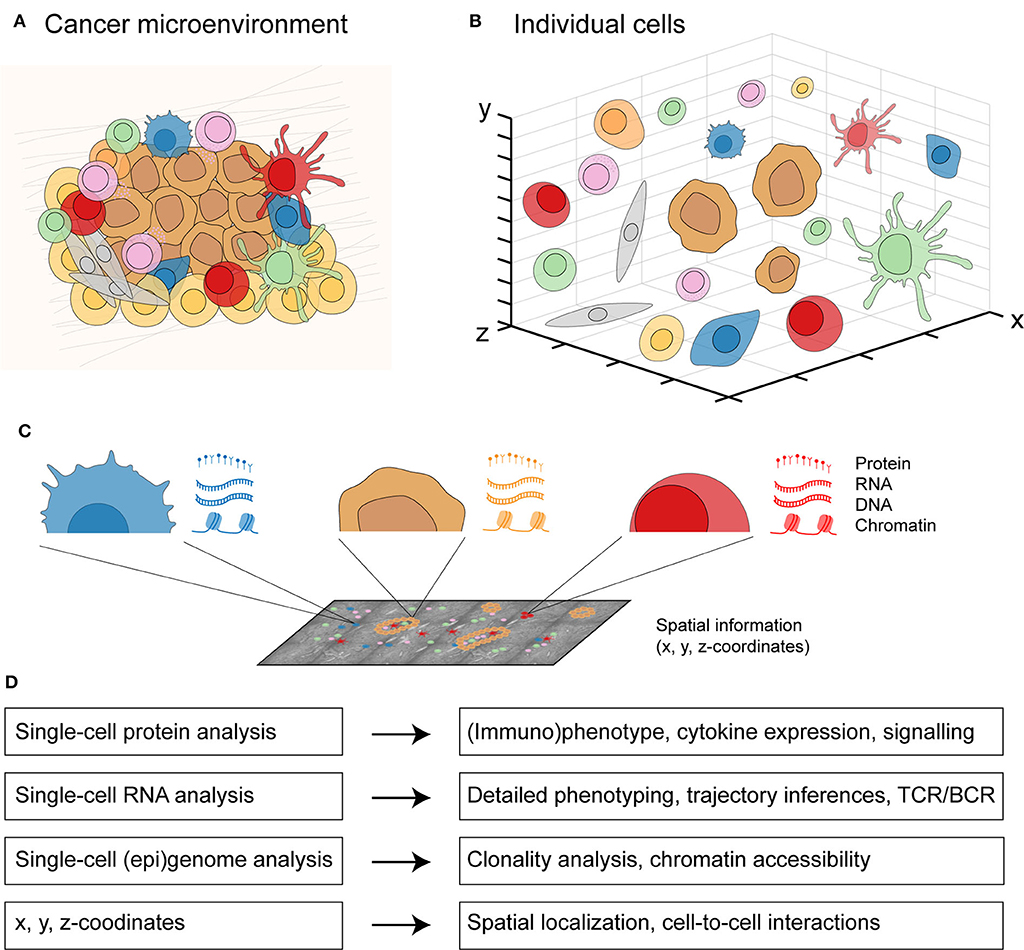
\includegraphics[width=0.7\columnwidth]{Chapter1/Figures/figure_1.jpeg}
    \caption{Approaches to study cell interactions in cancer (A) Characterisation of spatial organization of cells in a tumour. (B) Three-dimensional projection (e.g. sc-RNA-seq data) of individual cells after dissociation. (C) Measure each cell via multi-omics data including proteome, transcriptome, genome, epigenome and spatial location. (D) By integrating different layers of information for each cell, detailed profiling of the cancer environment is possible. (Adapted figure from \cite{de2020unraveling})}
    \label{fig:multimodal_approach_cci}
\end{figure}

While in some cases a single technique might be sufficient, more often the combination of single-cell multi-omics and imaging technologies are required to solve the complexity of cell communication in cancer (Fig.\ref{fig:multimodal_approach_cci}). In addition, we need more advanced technologies which allow the acquisition of molecular profiles from single cells without the need of dissociating them from their tissue context \cite{de2020unraveling}. 
% In fact, there are a few technologies which have been developed to enable single cell omics profiling without dissociation, many of them will be discussed in the following sections \ref{subsec:RNA_ISH}, \ref{subsec:ST_seq} and \ref{subsec:Spatial_proteomics}.

Similar to spatially resolved transcriptomics, spatial proteomics refers to the set of methods that use imaging technology for the visualization of proteins in their native cellular environment without the need for physical separation of cells or organelles before proteomic analysis. In addition to understanding the morphological context of RNAs, the spatial distribution of proteins is also equally important in studying cancer. The protein localization directly connects to protein function in health and disease. Being able to capture the localization of proteins and their dynamics at the cellular level is essential for a complete understanding of cell biology \cite{lundberg2019spatial}. 

Recent developments in flow cytometry, high-throughput microscopy and mass spectrometer have enabled to apply conventional protein study strategies in a spatially resolved context. The first wave of spatial proteomics methods used mass cytometric (MC) analysis. As an off-shoot from IHC/IF technology, MC-based spatial proteomic methods use antibodies to visualize the protein. An advantage of this type of analysis approach is that it can easily be used to study proteins in many different cell types. Two notable technologies have been developed that are based on the MC approach including Hyperion Imaging Mass Cytometry (IMC) as the pioneer and Multiplex Ion Beam Imaging (MIBI) as the direct competitor platform. Both of the methods use antibodies conjugated to stable metal isotopes. In IMC, after the tissue section is immobilized on slides. it is stained with panels of antibodies then it enters a laser ablation chamber where it is rasterized until it plumes. The aerosolized/ionized plumes of tissue are fed into time-of-flight mass spectrometer for analysis of isotope abundance.  There was a study that combined two technology of RNAscope and IMC workflow to interrogate the interplay between transcription and protein in the tissues \cite{schulz2018simultaneous}. Instead of using fluorophores, the RNAscope probes is modified to tag with metal. Thus mRNA and protein can be simultaneously measured in single cells. By using pure and rare-earth element isotopes, IMC can overcome the limitations of spectral overlap observed in IF and allow to quantify up to 38 tagged channels simultaneously. However, the use of lasers damages the tissues that are being scanned. MIBI can be used as an alternative approach to imaging histological sections labeled with isotope-tagged antibodies. Most of the steps for measuring protein levels using MIBI are quite similar to IMC. However, in MIBI secondary ion mass spectrometry is needed and  an (oxygen) ion beam is used instead of laser ablation to raster over the tissue. Subsequently, ions are analysed using mass spectrometer. While the MIBI only ablates a thin layer of the tissue (20-50nm) and cause fewer damages, the technology creates matrix effects and makes quantification more challenging \cite{bodenmiller2016multiplexed}. [...]

There exists another branch of technology called Mass Spectrometry Imaging (MSI) that characterises protein expression using mass spectrometer. Matrix‐Assisted Laser Desorption/Ionization (MALDI) tissue imaging is a technology using this approach and has been proven to be more versatile than MC. In MALDI, a laser and mass spectrometer are used to ablate the tissue and ionize the molecules. Eventually, the ionized molecules are fed to the spectrometer to determine the molecular weights \cite{caprioli1997molecular}.  This is performed in a label-free manner to measure the proteins present in the tissue. In this way MALDI is more suitable for the non-targeted experiments. However, there are also a number of limitations for MALDI or MSI in general such as lower spatial resolution, reduced sensitivity for larger protein, and low multiplexing capability. [...]

\begin{table}[ht]
\centering
\caption{Feature comparison of spatial proteomic technologies}
\begin{tabular}{||P{3cm} || P{3.5cm} || P{2cm} || P{2cm} || P{2cm} ||} 
 \hline
   & Staining IF   & \multicolumn{3}{c||}{Mass tagged antibodies} \\  [0.33ex] 
 \hline\hline
 Technologies & CycIF, CODEX, NanoString DSP  & IMC & MIBI & MALDI   \\ 
 \hline
 Resolution & $\sim$600$\mu$m-single cell  &  $\sim$1000$\mu$m & $\sim$260$\mu$m & 50-200$\mu$m \\
  \hline
 Repeat analysis  & Yes  &  No & Yes & Yes \\
  \hline
Maximum epitopes  & $\sim$60-96 & $\sim$40 & 40 & $<$10   \\ [1ex] 
 \hline
\end{tabular}
\label{table:SpatialProteomicComparison}
\end{table}

It is worth noting that protein visualization using fluorescence-based staining remains as another option. The advantages of using fluorescently conjugated antibodies to capture the presence of proteins are inherited from IHC and IF. These approaches involve iterative rounds of staining the protein with fluorescent probes which subsequently are detected by specialized instruments. There are multiple technologies for multiplexing fluorescence-based protein staining including NanoString GeoMx and co-detection by indexing (CODEX). In Nanostring DSP, a multiplexed cocktail of primary antibodies with  unique ultraviolet-photocleavable DNA oligos is used to target the proteins. After exposure to ultraviolet light from the GeoMX instrument, pools of released indexing oligos were hybridized to the optical barcodes and then read by another instrument (e.g NanoString nCounter or Illumina MiSeq) \cite{de2020unraveling, helmink2020b}. This enables to simultaneously detect up to 96 proteins and over 1000 RNA targets. CODEX have been developed by the inventor of MIBI and also uses a specialized instrument to convert images from fluorescence microscopes into a highly-multiplexed imaging systems. CODEX currently allows the detection of over 60 protein markers within the tissue by iteratively staining and scanning the tissue sections\cite{goltsev2018deep}. A disadvantage of CODEX, but also many other FISH-based technologies and IMC, is lack of signal amplification which results in under-detection of lowly abundant protein/gene markers. A comparative overview for three different approaches to perform spatial proteomic is available in Table \ref{table:SpatialProteomicComparison}. [...]

\subsubsection{}
\subsubsection{}
\subsection{Computational methods to study cell-cell interaction within spatial context}
Since distinct neighborhood of the tissue has been identified with one of the spatial methods then it’s natural to ask whether these cell types interact by their spatial proximity. Such information is lost in cell dissociation from scRNA-seq. The composition of tissue neighborhoods can be characterized with existing tools.
[...]
In stLearn , CellPhoneDB is used to identify L-R coexpression in neighboring spots, and the p-value of the coexpression is computed by permutation testing. Then regions with diverse cell types (from Seurat label transfering or cell type deconvolution) and L-R coexpression in neighboring spots are identified as regions where cells are likely to be signaling to each other. A similar strategy is used in Giotto. Giotto identifies cell type colocalization by labeling edges of the spatial neighborhood graph as homo- or heterotypic and permutes cell type labels to find whether the cell types are more or less likely to colocalize than expected from completely random cell type localization. L-R coexpression in neighboring cells on the spatial neighborhood graph from two cell types is identified and the p-values of the coexpression scores are computed by permutation testing, permuting locations of cells within each cell type. Within one cell type, Giotto uses classical DE (Student’s t-test, Wilcoxon rank sum test, limma, and permutation of spatial locations) to find DE genes between neighbors of cells of another cell type and non-neighbors.

In GCNG (Yuan and Bar-Joseph 2019), the spatial neighborhood graph is constructed as an edge connects a cell to its 3 nearest neighbors. Then both the gene count matrix and the normalized Laplacian of the neighborhood graph are fed into a graph convolutional neural network (GCN), which is trained on known L-R pairs. The GCN can then predict novel pairs of genes involved in signaling, and if trained on the direction of interaction in the L-R pairs, it can also predict the direction of causality in the novel pairs. With the cell-cell distance matrix, another optimal transport plan from ligands to receptors can be inferred, interpreted as how likely one cell communicates with another. A disadvantage of spatial neighborhood graph is that common ways of construction are somewhat arbitrary. For instance, k nearest neighbor is a common way to construct the graph, but this k is somewhat arbitrary, although cell signaling can occur over a distance with secreted ligands.

With a very different model, DIALOGUE identifies genes that may be involved in interactions between cell types. DIALOGUE aims to identify such concerted gene programs in each cell type. First, the gene expression data is projected into a lower dimensional space in which correlation between all pairs of cell types across niches is maximized, and the basis of this space is ordered in descending strength of correlation. This is similar to CCA, but with a penalty term to enforce sparsity in gene loading. Here the niche is a patch of cells in space with a predefined number of cells. Then each cell type has a rotation matrix that projects cells into this lower dimensional space, and different cell types from the same niche should be close to each other in this space.

Histocat's neighborhood analysis uses  basic statistical methods to find significantly enriched interactions between or within cell type. The pairwise interactions of every cell is defined by user (6 pixels). Using the cell segmentation masks as the representation of the cells, neighbour is defined as a pair of cells are within the pixel distance selected during the loading process. The pairwise interaction was compared to a random distribution using two individual one-tail permutation test within the same image. The test suggested how significant a pairwise interaction between two cell types was compared to random, and eventually suggested an interaction or an avoidance. The comparison to a matched randomized tissue for every individual image controls for both the distinct connectivity and the specific cell types in that tissue. 

\begin{equation}
\begin{split}
P_{lt} = \frac{ \sum(mean(permutation) \leq mean(real\_data) )}{number\_perm + 1} \\
P_{gt} = \frac{\sum(mean(permutation) \geq mean(real\_data) )}{number\_perm + 1}
\label{chap1:eq:02}
\end{split}
\end{equation}
Where $P_{gt}$ and $P_{lt}$ defined $P$ value for each tail, 
The absolute cell number or the size of the image does not have a direct effect on the neighborhood analysis, only the frequencies of cell types present and the relative quantities are important. 

squidpy is another analysis package that provides a thorough spatial analysis and visualisation of any given spatial -omic data. The squidpy packges is builts on   

Spatial variance component analysis (SVCA) (Arnol et al. 2019) models the expression of each gene of interest among the cells as a 0 mean Gaussian process. The covariance h
[...]
Despite the described experimental advances in imaging and sequencing technologies, there are limited computation approaches have been developed to enable and expand the analysis of the data. Most open-source tools that provide image-linked data analysis workflows were typically developed for low-plex fluorescence microscopy (e.g IHC and IF) and were not geared to apply in analysing of highly multiplexed measurements. There are some emerging open-source software tools that provide highly interactive graphic interfaces and are more user friendly graphic such as QuPath, CellProfiler and HistoCat. These open source software has an advantage of customising analysis modules which allow users to implement and optimise the analysis of their own. It is also worth noting that open-source software are widely popular among the research community. Thus, the user community and support are more available  than that\'s of commercial software. 

Meanwhile, there is a number of analysis packages that do not provide graphical interface but can control every functions inside such as Spatial Seurat, scanpy. The advantage of having control of analysis through script is that allows to scale up the amount of data easily. These packages are more suitable for bioiformatician and those who have computational background. However, they often abandon and undervalue spatial information while focus more on sc-RNAseq profile. It necessary to interrelate and utilise layers of information obtained from spatially resolved omic data. There is still lack of analysis software that can properly address the need for incorporate multiple type of data as well as provide the capability to scale up the analysis.


\label{subsec:ST_seq}


% \subsubsection{RNA in situ hybridization (ISH)}


% \subsubsection{Spatial proteomics}

\section{Research Objectives}
The rise of immunotherapy is substantially changing the cancer treatment paradigm \cite{dobosz2019intriguing}. However, less than $30\%$ patients respond to a single treatment type \cite{ott2017combination}. In addition, immunotherapy also associates with a variety of severe autoimmune-like side effects \cite{naidoo2015toxicities,bertrand2015immune}. These can be attributed to heterogeneity among single cells within the tissue. Technologically, single cell multimodal omics integration is recognized as method of the year for 2019 by Nature Methods \cite{teichmann2020method}. By simultaneously measuring multiple modalities, we can gain insight of different aspects of one cell at a time. Thus, it can greatly inform the discovery of relationships across cell types and relationships across -omics \cite{teichmann2020method}. The expansion of spatial omics data further improves our understanding about different angles of cell communication in cancer as well as the finding of rational immunotherapy agents. Since both discovery and translational research goals investigating cell communication rely on integration of spatial omics datasets, my PhD project that will be focused on implementing analysis methods to combine imaging and sequencing data to investigate intercellular communication.   
The overarching hypothesis of this project is: \textbf{a large number of cell-cell interactions in cancer can be identified and characterised by spatial omic data.}



\section{Thesis Overview}

Chapter 2: Spatial Transcriptomic and single cell RNA sequencing for cell-cell communication 

Cell-to-cell communication underscores a dynamic cellular ecosystem that develops, evolves, and responds to environmental factors. The implications and roles of cell-to-cell communication have been investigated extensively, particularly in cancer, using a wide range of in vitro and in vivo techniques, albeit at different scales and resolutions \cite{brucher2014cell}. Breakthroughs arising from discoveries in cell communication have led to important clinical applications. A classic example is the interaction via immune checkpoint proteins \cite{pardoll2012blockade}. Tumor cells, tumor infiltrating lymphocytes and tumor associated myeloid cells express inhibitory PD-L1/CTLA4 ligands to engage PD-1 receptors on cytotoxic T cells and CD80/86 receptors on myeloid cells, effectively blocking immune activation against the tumor cells. The discovery has led to applications of using monoclonal antibodies that specifically target this ligand-receptor (L-R) interaction as a form of immunotherapy, allowing immune cells to suppress cancer growth \cite{weiner2012antibody}. Therapies targeting these two pairs of ligand-receptors have transformed the management of several cancers, including melanoma, renal cell carcinoma, bladder cancer, head and neck cancer, and many others \cite{ott2017combination}. Notably, often less than 20\% of patients respond to a single immunotherapy, including common cancer types like breast, colon and prostate cancer \cite{ott2017combination}, and hence the urgent need to combine therapies, for example by using antibodies against PD-L1, CTLA-4 and/or PD-1 \cite{ott2017combination}. However, mechanisms of action for combinational immunotherapies remain elusive \cite{wei2019combination} and the number of current druggable targets for cancer-immune cell interaction is extremely limited, compared to the large repertoire of over 2,000 known ligands and receptors. Therefore, research to explore and advance understanding of known and new ligand-receptor pairs in the context of tumor-immune cell interaction within a tumor is extremely important for the further development of immunotherapies \cite{weiner2012antibody, helmy2013cancer}. 

Most ligand-receptor (L-R) interaction research so far has been relying on the use of fluorescently-conjugated antibody-based methods, that are only able to assess protein levels of a few target molecules and results are often based on a small number of cells at a time. Whole-transcriptome analysis, especially methods using single-cell RNA-seq (scRNA-seq) with gene expression profiles at single cell level, provide a means towards high-throughput L-R screening assays \cite{browaeys2020nichenet, efremova2020cellphonedb}. However, these transcriptomics-based methods do not assess cellular communication in a tissue context, where interactions happen only between neighbour cells but not between distant cells. Often, these methods result in a large number of false positive predictions. Spatial transcriptomics (ST-seq) overcomes these limits and enable the study of (target) gene expression in undissociated tissue sections, maintaining tissue integrity \cite{salmen2018barcoded}. ST-seq measures barcoded gene expression in spots printed onto a functional glass slide \cite{salmen2018barcoded}, which captures mRNA released from a tissue section, preserving the cell morphology.  ST-seq has been applied to study the gene expression landscape of tissues and diseases, such as prostate cancer \cite{berglund2018spatial, ji2020multimodal}, pancreatic cancer \cite{moncada2019integrating}, melanoma \cite{thrane2018spatially}. However, ST-seq still has not achieved single-cell resolution per spatial spots (1-50 cells/spot), and the number of cells as well as the transcriptome quality that can be captured in each spot depend on the tissue context. These shortcomings of ST-seq can be overcome by a targeted RNA in situ hybridization (RNA-ISH) approach to visualize the cell interaction through detecting L-R at a single cell level. The RNAscope HiPlex assay (ACD Bio) has been developed based on the RNA-ISH technique and improved on the signal amplification and background suppression process compared to the previous version, allowing for visualization and detection of mRNA at near single molecule sensitivity. The technology allows researchers to simultaneously detect up to 12 single target genes on the same tissue section through fluorophore cleavage steps. Extending from measuring RNA, we implemented another technique to detect protein, covering the whole tissue and at subcellular resolution. Opal multiplex IHC can measure 4-7 proteins on the same tissue. While the experimental frameworks are accessible, all the scRNA-seq, ST-seq, RNAscope and IHC data require computational analyses to quantitatively process the sequencing and imaging data so that cell-cell interactions can be inferred from and compared across datatypes. 

\begin{enumerate}[align=left]
    \item[\textbf{2.1}] Use ST-seq data to study cancer-immune cell communication.
    \item[\textbf{2.2}] Validate the findings from ST-seq using other target-specific technologies.
\end{enumerate}
This motivation of this chapter derives from the idea to utilise the ST-seq data to study cell-cell interaction throughout the tissue. I have been developing analysis methods to detect the possible cell-cell interaction through ligand-receptor means, across neighboring spots in ST data. To validate the finding from ST-seq, I adopt the RNA ISH with RNAscope to capture the presence of two pairs of markers that are involved in ligand-receptor signalling. Additional validation of the RNAscope assessment, digital droplet PCR is used to quantitatively measuring the molecules from tissues for comparison with RNAscope results.      

Chapter 3: Spatial proteomic for mapping cell types and identifying interactions across tissues
\begin{enumerate}[align=left]
    \item[\textbf{3.1}] Use spatial proteome profiling data to inform the cell types composition in the tissues.
    \item[\textbf{3.2}] Correlate cell types with the with their spatial context to understand physiological state of the tumour microenvironment.
    \item[\textbf{3.3}] Quantitative and qualitative measurements
\end{enumerate}
As described in section \ref{subsec:motivation}, multimodal omic measurement offers a holistic view of cells in their native context. Spatial proteomics can be a complementary method that can link the protein expression levels to cellular transcriptomes. However, the availability of analysis workflows and methods are still limited. This aim will focus on developing novel machine learning analysis methods of spatial proteomic data to shed light into cell-cell communication at protein level. In addition, the aim is also to identify cell types using protein markers and their interaction across the tissue microenvironment.             

Chapter 4: The association between tumour spatial structures and clinical diagnostics or subtype classification
\begin{enumerate}[align=left]
    \item[\textbf{4.1}] The variation of tumor microenvironment structures in skin cancer
    \item[\textbf{4.2}] The tumor microenvironment analysis across patients in colorectal cancer samples
    % \item[\textbf{Aim 4.}] Quantitative and qualitative measurements
\end{enumerate}
Chapter 2 and Chapter 3 uses spatial-omic data to study cell interaction in tissue, chapter 4 will aim to alleviate from applying the methods developed in the Aim 1 and 2 to multiple patient samples. Building upon what has been discussed, the ultimate goal is to visually understand cell interactions, especially immune-cancer cell interactions. Thus, I will demonstrate the power of integrative analysis methods and workflows on two specific cancer types including skin cancer and colorectal cancer.

Chapter 5: Discussion and future plan
\begin{enumerate}[align=left]
    \item[\textbf{5.1}] Application of analysis pipeline to study multiplexed imaging data.
    \item[\textbf{5.2}] Closing remark
\end{enumerate}

% \bibliographystyle{elsarticle-num}
% \typeout{}
% \bibliography{./References/Bibliography}
% \printbibliography[heading=subbibliography]